\chapter{Renormalization Group}
\label{RG}
Since it is central for this thesis to see how the renormalization group (RG) affects on the SDC, another preliminary we need before the computaion is the concept of renormalization group and how we can carry out the calculations. In this chapter, first we will have introductions to the renormalization group (RG) starting from a review of the generating functional to the beta function, or the RG equations. Understanding the basics of RG, we will provide a specific method for our later computation, named Heat Kernel expansion.

\section{Focused Review of Generating Functional}
Consider a theory with n fields $\phi^{i} (x)$, $i = 1, \dotso , n$, governed by a classical action $S[\phi]$, and suppose computing its correlation functions:
\begin{align}
    G^{i_{1}, \dotso , i_{n}} (x_{1}, \dotso ,x_{n} ) := \mel{\Omega _{f}}{T[\phi^{i_{1}}(x_{1}) \dots \phi^{i_{n}} (x_{n})]}{\Omega _{i}}
\end{align}
where $\ket{\Omega}$ stands for the ground state in the past or future, and T indicates time ordering. We can extract general observables of the system such as scattering amplitudes from them. By introducing the generating functional $Z[J]$, we can deal with such correlators at onece. Definition of $Z[J]$ is:
\begin{align}
    Z[J] := \sum_{n=0} ^{\infty} \frac{i^{n}}{n!} \int d^{4}x_{1} \dotso d^{4}x_{n}   G^{i_{1}, \dotso , i_{n}} (x_{1}, \dotso ,x_{n} ) J_{i_{1}}(x_{1}) \dots J_{{i_{n}}}(x_{n})
\end{align}
then each correlation function can be in a form by functional differentiation:
\begin{align}
    G^{i_{1}, \dotso , i_{n}} (x_{1}, \dotso ,x_{n} ) = (-i)^{n} (\frac{\delta^{n}Z[J]}{\delta J_{i_{1}}(x_{1}) \dots \delta J_{i_n} (x_{n})}) _{J=0}
\end{align}
The generating functional is useful because it is a simple expression in terms of path integral formalism. Such simplicity means not only the easiness to be computed but also practically that it is relatively straightforward to compute perturbatively in terms of Feynman diagrams. 
\begin{align}
    G^{i_{1}, \dotso , i_{n}} (x_{1}, \dotso ,x_{n} ) = \int \mathcal{D} \phi e^{iS[\phi]} \phi^{i_1} (x_{1}) \dots \phi ^{i_{n}}(x_n)
\end{align}
where the integration measure is:
\begin{align}
    \int \mathcal{D} \phi = \prod_{x^{\mu}} \int d\phi(x)
\end{align}
The special case $n=0$ is the typical example for which
\begin{align}
    \braket{\Omega _{f}}{\Omega _{i}} = \int \mathcal{D} \phi e^{iS[\phi]}
\end{align}
Using the definition, we can obtain the following expression for the generating functional:
\begin{align}
    Z[J] = \int \mathcal{D} \phi exp\lbrace iS[\phi] + i \int d^{4}x \phi^{i} (x) J_{i} (x) \rbrace
\end{align}
and immediately find:
\begin{align}
    Z[J=0] = \braket{\Omega _{f}}{\Omega _{i}}
\end{align}

\subsubsection{Semiclassical Evaluation}
Expand the action about a classical background so that:
\begin{align}
    \phi(x) = \varphi_{\text{cl}} (x) + \tilde{\phi}(x) 
\end{align}
where $\varphi_{\text{cl}}$ fulfills:
\begin{align}
    \label{eq:semi}
    \eval {\fdv{S}{\phi}}_{\phi = \varphi_{\text{cl}}} + J = 0
\end{align}
Suppose we have an action $S_{j}[\phi] := S[\phi] + \int d^{4}x (\phi ^{i} J_{i})$, and want to write it in a form:
\begin{align}
    S_{j} [\varphi_{\text{cl}} + \tilde{\phi}] = S_{J}[\varphi _{\text{cl}}] + S_{2} [\varphi _{\text{cl}}, \tilde{\phi}] + S_{\text{int}}[\varphi_{\text{cl}}, \tilde{\phi}]
\end{align} 
where:
\begin{align}
    S_{2} = -\int d^{4} x \tilde{\phi^{i}}\Delta _{ij}(\varphi_{\text{cl}}) \tilde{\phi ^{j}}
\end{align}
being the quadratic part in the expansion for some differential operator $\Delta _{ij}$. $S_{\text{int}}$, namely interaction term, contains higher order terms in $\tilde{\phi^{i}}$. Notice that since the background field satisfies eq.\ref{eq:semi}, there will be no linear terms. \\
\indent Then the expression inside the above path integral can be expanded as:
\begin{align}
    \exp \lbrace iS[\phi] + i\int d^{4}x \phi^{i}J_{i} \rbrace = \exp \lbrace iS_{J}[\varphi_{\text{cl}}]+ iS_{2} [\varphi_{\text{cl}}, \tilde{\phi}] \rbrace \sum_{r=0}^{\infty} \frac{1}{r!} (iS_{\text{int}}[\varphi_{\text{cl}},\tilde{\phi}])^{r}
\end{align}
This will be followed by the graphical representation of any correlators. Gaussian integrals involve integrands which are powers of fields:
\begin{align}
    \int \mathcal{D} \tilde{\phi} e^{i\tilde{\phi}^{i}\Delta _{ij} \tilde{\phi}^{j}} \tilde{\phi}^{k_{1}}(x_{1}) \dots \tilde{\phi}^{k_{n}} (x_{n}) \propto (\text{det}^{-1/2} \Delta) [(\Delta ^{-1})^{k_{1}k_{2}} \dots (\Delta ^{-1})^{k_{n-1}k_{n}} + (\text{permutations})]
\end{align}
for even $n$, while the integrand vanishes if $n$ is odd. The combinatorics in an integral correspond to the combinatorics of all posiible ways to connect graphs whose internal lines represent factors of $\Delta ^{-1}$ and vertices to interactions within $S_{\text{int}}$. In this language, $Z[J]$ denotes the sum over all vacuum graphs with no external lines. Some leading perturbative contributions to the generating functional are:
\begin{align}
    Z[J] = N (\text{det}^{-1/2} \Delta)[ 1+
    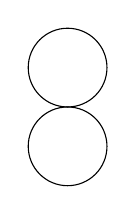
\begin{tikzpicture}
        \draw (0,0) circle (0.5);
        \draw (0,-1) circle (0.5);
    \end{tikzpicture}
    ]
\end{align}
where solid lines are propagators and black dots represent interactions appear in $S_{\text{int}}$. \\ This indeed includes all graphs containing those that are disconnected. Such graphs are disconnected in the sense that it is not possible to get between any pair of vertices along some sequence of internal lines. \\
\indent Those expansions here are not practical yet in order to carry out the explicit computaions because of the appearance of the background field in the propagator $\Delta _{ij}(x,y) = \frac{\delta^{2}S}{\delta \phi ^{i}(x) \delta \phi ^{j}(y)}$. For example, for a scalar field wit a scalar potential $U(\phi)$, we have $\Delta(x,y) = [-\square + U'' (\varphi)]\delta ^{4} (x-y)$. This is easily inverted in momentum space if $\varphi$ is constant, but is not straightforward to invert for arbitrary $\varphi(x)$. Such a problem is often addressed by expanding in powers of $J_{i}(x)$ so that path integral is evaluated as a semiclassical expansion about a simple backgroud configuration $\varphi _{\text{cl}}^{i}$ which satisfies:
\begin{align}
    \eval{\fdv{S}{\phi ^{i}}}_{\phi = \varphi _{\text{cl}}} = 0
\end{align}
By doing this, for the modified expansion the term $\phi^{i} J_{i}$ in the exponent of the integrand is viewed as an interaction. This is linear in $\phi ^{i}$, so it corresponds to a tadpole contribution, with the line ending in a cross whose Feynman rule is $J_{i}(x)$.

\subsection{Connected Correlation}
Instead of dealing with all graphs including both connected and disconnected, it is usually useful to work with a generating functional $W[J]$ whose graphical representaion contains only connected ones. This is achieved by defining as $Z[J] := \exp \lbrace iW[J] \rbrace$, because taking logarithm means subtracting the disconnected graphs. This leads:
\begin{align}
    \label{eq:W}
    \exp \lbrace iW[J] \rbrace = \int \mathcal{D} \phi \exp \lbrace iS[\phi] + i\int d^{4}x \phi ^{i} J_{i} \rbrace 
\end{align}
Then corresponding correlation functions are given:
\begin{align}
    \expval{T[\phi ^{i_{1}}(x_{1}) \dots \phi ^{i_{n}}(x_{n}) ]} := (-i)^{n-1} \eval{\frac{\delta ^{n}W[J]}{\delta J_{i_{1}}(x_{1}) \dots \delta J_{i_{n}}(x_{n})}} _{J=0}
\end{align}

\subsection{The 1-Particle Irreducible Action}
As discussed, $Z[J] = \exp \lbrace iW[J] \rbrace$ can be thought of as the 'in-out' vacuum amplitude with a current $J_{i}$. In addition, the current can be interpreted as being responsible for varying the expectation value of the field since at $J_{i}  = 0$:
\begin{align}
    \varphi^{i} (x) := \expval{\phi^{i}(x)} = \fdv{W}{J_{i} (x)}
\end{align}
But it is often more simple to have the vacuum-to-vacuum amplitude expressed as in terms of a functional of the expectation value $\varphi ^{i}$. This can be done through a Legendre transform. In order to perform Legendre transform, we may define:
\begin{align}
    \Gamma [\varphi] := W[J] - \int d^{4}x \varphi ^{i}J_{i}
\end{align}
here $J_{i}(x)$ is a functional of $\varphi ^{i}(x)$. Then we have a relation:
\begin{align}
    \fdv{\Gamma}{\varphi^{i}(x)} = -J_{i}(x)
\end{align}
It shows that the expectation value for the system with $J_{i}=0$ is a stationary point of $\Gamma[\varphi]$. Therefore, the relation between $\Gamma[\varphi]$ and $\expval{\phi^{i}}$ is to the one between the classical action and a classical background configuration. 
\subsubsection{Semiclassical Expansion}
Now consider about the computation of $\Gamma[\varphi]$ within perturbation theory. From eq.\ref{eq:W}, we may have:
\begin{align}
    \begin{split}
        \exp \lbrace i\Gamma[\varphi]\rbrace &= \exp \lbrace iW[J] - i\int d^{4}x \varphi^{i} J_{i} \rbrace \\
        &= \int \mathcal{D} \phi \exp \lbrace iS[\phi] + i \int d^{4}x (\phi ^{i} - \varphi ^{i})J_{i} \rbrace \\
        &= \int \mathcal{D} \tilde{\phi} \exp \lbrace iS[\varphi + \tilde{\phi}]+ i\int d^{4}x \tilde{\phi} ^{i} J_{i}
    \end{split}
\end{align}
in the last line we changed the integration variable as $\phi ^{i} \rightarrow \tilde{\phi}^{i} := \phi ^{i} - \varphi ^{i}$. Expanding the action inside the path integral about $\phi^{i} = \varphi ^{i}$:
\begin{align}
    S[\varphi + \tilde{\phi}] = S[\varphi] + S_{2} [\varphi, \tilde{\phi}] + S_{\text{int}}[\varphi,\tilde{\phi}]
\end{align}
This is a similar expression we had before except the term linear in $\tilde{\phi}^{i}$:
\begin{align}
    S_{\text{int}}[\varphi,\tilde{\phi}] = \int d^{4}x [\eval{\fdv{S}{\phi^{i}}(x)}_{\phi=\varphi} + J_{i}(x)] \tilde{\phi}^{i}(x)
\end{align}
which does not vanish since $\delta \varphi^{i} := \varphi ^{i} - \varphi_{\text{cl}}^{i} \neq 0$. However, $\delta\varphi^{i}$ is perturbatively so small that it would be within $S_{\text{int}}$, expanded within the integrand, and not kept in the exponential. The expantion eventually becomes:
\begin{align}
    e^{i\Gamma[\varphi]} = e^{iS[\varphi]} \int \mathcal{D}\tilde{\phi} e^{iS_{2}[\varphi,\tilde{\phi}]}\sum _{r=0}^{\infty} \frac{1}{r!}(iS_{\text{int}}+ i S_{\text{lin}})^{r}
\end{align}
and then:
\begin{align}
    \label{eq:Gamma}
    \Gamma[\varphi] = S[\varphi] + \frac{i}{2}\ln \det \Delta + (\text{more than 1-loops})
\end{align}
The first two terms in eq.\ref{eq:Gamma} are the classical and one-loop contributions respectively, though the last contains the sum over all Feynman graphs with two or more loops. \\
\indent Since $S_{\text{lin}}$ is linear term in $\tilde{\phi}^{i}$, its Feynman rule is as seen before, which inserts a tadpole contribution proportional to $\fdv{S}{\varphi ^{i}} + J_{i}$. Notice that evaluationg at $J_{i} = -\fdv{\Gamma}{\varphi ^{i}}$, eq.\ref{eq:Gamma} gives:
\begin{align}
    \begin{split}
    \fdv{S}{\varphi^{i}(x)} + J_{i}(x) &= \fdv{\varphi^{i}(x)} (S[\varphi] - \Gamma[\varphi])\\
    &= - \fdv{\varphi^{i}(x)} [\frac{i}{2} \ln \det \Delta + (\text{more than 1-loops})] \\
    & = -(\text{sum of tadpole graphs})
    \end{split}
\end{align}
Therefore, we can manipulate without knowing expression for $\Gamma[\varphi]$. $J_{i} =-\fdv{\Gamma}{\varphi}$ imdicates that all graphs involving explicit dependence on $J_{i}$ cancel all graphs which can be split into two disconnected graphs. In this language, a graph which cannot be separated into tow pieces is called 1-particle irreducible (1PI). Thus, $\Gamma[\varphi]$ can be obtained by evaluating only 1PI graphs. Therefore, $\Gamma[\varphi]$ is often called the generator of 1PI correlations, or 1PI action. In semiclassical expansion, eq.\ref{eq:Gamma} is computed as a sum of 1PI connected graphs without external lines. \\
\indent Viewing $\Gamma[\varphi]$ only involves 1PI suggests alternative way in which $\Gamma[\varphi]$ generalizes the classical action. In a perturbative expansion the leading approximation is the leading term in $\Gamma[\varphi] \approx S[\varphi]$. Considering scattering amplitudes, this amounts to summing the tree level graphs from vertices from the classical interactions in $S_{\text{int}}$. On the other hand, suppose computing Feynman graphs by the expansion of $\Gamma[\varphi + \tilde{\phi}]$ to obtain the propagators and vertices. For this, loops for any correlators with Feynman rules for $S[\varphi]$ is same as the quantities given by summing all tree graphs made from the Feynman rules for $\Gamma[\varphi]$. Thus, the full quantum amplitude can be found by computing with $\Gamma[\varphi]$ within the classical approxiamtion. 

\section{Wilsonian Effective Action}
Now let us consider a field theory with characteristic (large) energy scale $M$, and suppose we want to study physics at a lower energy regime namely $E \ll M$. This is precisely the situation the EFTs are useful. The full theory is defined in terms of the path integral, and we can extract observables from calculating the correlator:
\begin{align}
    \mel{0}{T[\phi(x_{1}) \dotso \phi(x_{n})]}{0} = \frac{1}{Z}\int \mathcal{D} \phi e^{iS[\phi]} \phi(x_{1}) \dots \phi(x_{n})
\end{align}
with the integration measure is:
\begin{align}
    \int \mathcal{D}\phi = \prod_{x^{\mu}} \int d\phi(x)
\end{align}
and
\begin{align}
    Z = \int \mathcal{D}\phi e^{iS[\phi]}
\end{align}
Then consider what happend as we try to perform the path integral by integrating those modes first with energy between $\Lambda _{0}$ and $\Lambda < \Lambda_{0}$. We can split a generic field $\phi(x)$ as:
\begin{align}
    \begin{split}
        \phi(x) &= \int _{\abs{p} \le \Lambda_{0}} \frac{d^{d}p}{(2\pi)^{d}} e^{ip\dot x} \tilde{\phi}(p) \\
        &= \int _{\abs{p} \le \Lambda} \frac{d^{d}p}{(2\pi)^{d}} e^{ip\cdot x} \tilde{\phi}(p) + \int _{\Lambda < \abs{p} \le \Lambda _{0}} \frac{d^{d}p}{(2\pi)^{d}} e^{ip\cdot x} \tilde{\phi}(p) \\
        & := \varphi (x) + \chi (x)
    \end{split}
\end{align}
where $\varphi(x)$ and $\chi(x)$ are low- and high-energy part of the field respectively. Thus the path integral measure can be rewritten as:
\begin{align}
    \mathcal{D}\phi = \mathcal{D} \varphi \mathcal{D} \chi
\end{align}
into a product of measures over low- and high-energy modes. Since we are now interested in low-energy physics, we just need to compute the correlation function:
\begin{align}
    \mel{0}{T[\varphi(x_{1}) \dotso \varphi(x_{n})]}{0} = \frac{1}{Z} \int \mathcal{D} \varphi \int \mathcal{D} \chi e^{iS[\varphi + \chi]} \varphi(x_{1}) \dotso \varphi(x_{n})
\end{align}
Then we define a Wilsonian effective action at scale $\Lambda$ $S_{\Lambda}[\varphi]$ as follows:
\begin{align}
    e^{iS_{\Lambda}[\varphi]} := \int \mathcal{D}\chi e^{iS[\varphi + \chi]}
\end{align}
and we have chosen $\Lambda < M$ to integrate out the physics associated with $M$. $S_{\Lambda} [\varphi]$ is non-local n scales $\Delta x^{\mu} \gtrsim \frac{1}{\Lambda}$, that is, the Lagrangian is not just a polynomial of the fields or their derivatives evaluated at a single point in spacetime, since high-energy fluctuations have been integrated out. Expanding the non-local action a series of local operators:
\begin{align}
    S_{\Lambda} [\varphi] &= \int d^{d}x \mathcal{L}_{\Lambda}^{\text{eff}}(x) \\
    \mathcal{L}_{\Lambda}^{\text{eff}(x)} &= \sum_{i} g_{i}\mathcal{O}_{i}(x)
\end{align}
here $\mathcal{L}_{\Lambda}^{\text{eff}}(x)$ is an effective Lagrangian at scale $\Lambda$.  It is an infinite sum over local operators $\mathcal{O}_{i}$ allowed by symmetries. The coefficients gi are referred to as Wilson coefficients.
\subsection{Running Couplings and Their Beta-functions}
It is important to notice that the partition function:
\begin{align}
    Z_{\Lambda} (g_{i} (\Lambda)) = \int _{\le \Lambda} \mathcal{D} \phi e^{-iS_{\Lambda}[\phi]}
\end{align}
obtained from the effective action at scale $\Lambda$ is exactly the same as the one we started with:
\begin{align}
    Z_{\Lambda}(g_{i}(\Lambda)) = Z_{\Lambda_{0}}(g_{i0};\Lambda_{0})
\end{align}
because we are just computing the remaining integrals over the low-energy modes. Particularly, as the scale is lowered infinitesimally, this becomes:
\begin{align}
    \label{eq:rgpf}
    \Lambda\dv{Z_{\Lambda}(g)}{\Lambda} = (\eval{\Lambda \pdv{\Lambda}}_{g_{i}} + \Lambda\pdv{g_{i}(\Lambda)}{\Lambda} \eval{\pdv{g_{i}}}_{\Lambda})Z_{\Lambda}(g) = 0
\end{align}
Eq.\ref{eq:rgpf} is known as the renormalization group equation for the partition function. It is claiming that as we change the scale by integrating out modes, the couplings in the effective action $S_{\Lambda}$ vary to account for the change in the degrees of freedom over which we take the path integral so that the partition function is indeed independent of the scale at which we define our theory, provided this scale is below our initial cut-off scale $\Lambda_{0}$. Since the running of couplings is so important, it has a specific name and we can define the beta-function $\beta _{i}$ of the coupling $g_{i}$ to be the derivative with respective to the logarithm of the scale:
\begin{align}
    \beta_{i} := \Lambda\pdv{g_{i}}{\Lambda} = \pdv{g_{i}}{\ln \Lambda}
\end{align}


\subsection{1PI for Wilsonian Action}
Here let us consider the 1PI for a Wilsonian effective action $S_{\Lambda} [\varphi]$ following the procedure in previous section. To begin with, for our convinience by the Wick rotation we may have:
\begin{align}
    S_{\Lambda}[\varphi] := iS_{E,\Lambda}[\varphi]
\end{align}
and from now on we will just write this as $S_{\Lambda}[\varphi]$ unless it makes serious confusions. Then the generating functional for the Green functions of a field $\varphi$ in the path integral representaion is:
\begin{align}
    \begin{split}
        Z[J] &= \int \mathcal{D}\varphi \exp (-S_{\Lambda} [\varphi] - \int d^{d}x J(x)\varphi(x)) \\
        & = \int \mathcal{D} \varphi \exp (-\int d^{d}x (\mathcal{L} [\varphi(x)] + J(x)\varphi(x)))
    \end{split}
\end{align}
with an external source $J(x)$. Suppose then that a field $\varphi (x)$ can be splitted into two pieces: a classical background $\zeta(x)$ and a quantum fluctuations $\eta (x)$ so that:
\begin{align}
    \varphi(x) = \zeta(x) + \eta(x)
\end{align}  
with a condition $\eval{\fdv{S}{\varphi}} _{\varphi = \zeta} + J(x) = 0$ is satisfied. Then the expansion of the action around the backgroud gives:
\begin{align}
    \label{eq:expand}
    \begin{split}
    \int d^{d} x  (\mathcal{L}[\varphi(x)] + J(x) \varphi(x) ) = & \int d^{d}x  (\mathcal{L}[\zeta(x)] + J(x)\zeta(x))  \\
    + & \int d^{d} x (\eval{\fdv{\mathcal{L}}{\varphi}} _{\phi = \eta} + J(x)) \eta(x) \\
    + & \frac{1}{2} \int d^{d}x d^{d}y \eval {\frac{\delta ^{2} \mathcal{L}}{\delta \varphi(x) \delta \varphi(y)}} _{\varphi = \zeta} \eta(x)\eta(y) \cdots 
    \end{split}
\end{align}
The second term of eq.\ref{eq:expand} is identically zero due to the equation of motion. Then the generating functional can be in the form:
\begin{align}
    Z[J] = e^ {\qty (-\int d^{d}x (\mathcal {L} [\zeta (x)] + J(x) \zeta (x)))} \int \mathcal {D} \eta e^{- \frac{1}{2} \int d^{d}x d^{d}y \eval {\frac{\delta ^{2} \mathcal{L}}{\delta \varphi(x) \delta \varphi(y)}} _{\phi = \zeta} \eta(x)\eta(y) \cdots}
\end{align}
because the first integral in eq.\ref{eq:expand} has nothing to do with the fluctuation $\eta(x)$. Notice that the remaining path integral over $\eta$ is of Gaussian form and can be computed explicitly:
\begin{align}
    Z[J] = e^ {\qty (-\int d^{d}x (\mathcal {L} [\zeta (x)] + J(x) \zeta (x)))} \qty (\text{det} \frac{\delta ^{2} \mathcal{L}}{\delta \varphi(x) \delta \varphi(y)})^{-1/2} + \cdots
\end{align}
A generating functional $Z[J]$ takes the form $Z[J] = e^{-W[J]}$, then, with an identity $\text{det} \mathcal{A} = e^{\text{Tr} \ln \mathcal{A}}$:
\begin{align}
    W[J] = \int d^{d}x (\mathcal {L} [\zeta (x)] + J(x) \zeta (x)) + \frac{1}{2} \text{Tr} \ln \frac{\delta ^{2} \mathcal{L}}{\delta \varphi(x) \delta \varphi(y)} + \cdots
\end{align}
Performing a Legendre transformation in order to compute the effective action $\Gamma[\varphi]$:
\begin{align}
    \Gamma[\zeta] &= W[J] - \int d^{d} x J(x)\zeta(x) \nonumber \\
    & = \int d^{d}x \mathcal{L} [\zeta(x)] + \frac{1}{2} \text{Tr} \qty[\ln \frac{\delta ^{2} \mathcal{L}}{\delta \varphi(x) \delta \varphi(y)}] + \cdots
\end{align}
The first term is apparently the classical action. Thus the one-loop effective action is given:
\begin{align}
    \label{eq:2.8}
    \Gamma_{\text{1-loop}} [\varphi] = \frac{1}{2} \text{Tr} \qty[\ln \frac{\delta ^{2} \mathcal{L}}{\delta \varphi(x) \delta \varphi(y)}]
\end{align}
The divergent part of eq.\ref{eq:2.8} is the same as the counter-terms, i.e. the action at a renormalized scale. Therefore, it is necessary to be able to carry out this trace in some ways in order to find the beta functions. Here we will adopt the method of Heat Kernel expansion. 

\section{Heat Kernel Expansion}
\subsection{General Formalism}
For the manipulation of the trace, introduce the heat kernel:
\begin{align}
    K(t;x,y;D) = \mel{x}{e^{-tD}}{y}
\end{align}
such that it satisfies the heat conduction equation:
\begin{align}
    (\partial _{t} + D_{x})K(t;x,y;D) = 0
\end{align}
with an initial condition:
\begin{align}
    K(0;x,y;D) = \delta (x-y)
\end{align}
For instance, for a kernel for $ D = - \Delta$:
\begin{align}
    K(t;x,y;-\Delta) = (4\pi t)^{-d/2} \text{exp} ^{\qty (-\frac{(x-y)^2}{4t})}
\end{align}
and for $D = D_{0}= -\Delta +m^2 $:
\begin{align}
    K(t;x,y;D) = (4\pi t)^{-d/2} \text{exp}^{ \qty (-\frac{(x-y)^2}{4t} - tm^2)}
\end{align}
For a general D, $K(t;x,y;D_{0})$ still describes the leading singularity at $t \to 0$:
\begin{align}
    K(t;x,y;D) = K(t;x,y;D_{0}) (1 + tb_{2} (x,y) + t^{2} b_{4}(x,y) + \cdots)
\end{align}
Coefficients $b_{k} (x,y)$ are regular in the limit $y \to x$, and called the heat kernel coefficients. \\
\indent It is needed to compute the functional:
\begin{align}
    \Gamma_{\text{1-loop}} = \frac{1}{2} \Tr \ln D
\end{align}
where;
\begin{align}
    D = \frac{\delta^2 \mathcal{L}}{\delta \phi \delta \phi} 
\end{align}
But for each positive eignevalue $\lambda$ of the operator $D$, an identity is:
\begin{align}
    \ln \lambda = -\int _{0} ^{\infty} \frac{dt}{t} e^{-t\lambda}
\end{align}
Then eq.\ref{eq:2.8} can be rewritten:
\begin{align}
    \Gamma _{\text{1-loop}} = -\frac{1}{2} \int _{0}^{\infty} \frac{dt}{t} K(t,D)
\end{align}
where 
\begin{align}
    K(t,D) = \Tr e^{-tD} = \int d^{d} x \sqrt{g} K(t;x,x;D)
\end{align}
To see a UV divergence, introduce a cut-off at $t=\Lambda ^{-2}$, and compute a part of $\Gamma _{\text{1-loop}}$ which diverges in the limit $\Lambda \to 0$:
\begin{align}
    \begin{split}
    \Gamma _{\text{1-loop}} ^{\text{div}} =&  -(4\pi)^{-d/2} \int d^{d} x \sqrt{g} [ \sum_{2(j+l)< d} \Lambda ^{d-2j-2l} b_{2j}(x,x) \frac{(-m^{2})^{l} l!} {d-2j-2l}  \\
    &+ \sum_{2(j+l) =d} \ln \Lambda (-m^{2})^{l} l! b_{2j} (x,x) + \order {\Lambda ^{0}} ] 
    \end{split}
\end{align}
It can be seen that the UV divergence in the one-loop effective action are defined by finitely many heat kernel coefficients $b_{k} (x,x)$ with $k<d$. \\
\indent Moreover, suppose the operator $D$ is in a form:
\begin{align}
    D = -(g^{\mu \nu} \Delta _{\mu} \Delta _{\nu} + E)
\end{align}
according to %\ref{},
the trace can be expanded as:
\begin{align}
    \Tr e^{-tD} = \sum _{k \ge 0} t^{(k-d)/2} a_{k}
\end{align}
where
\begin{align}
    a_k = (4\pi)^{-d/2} \int d^{d}x \sqrt{g} b_{k}(x,x)
\end{align}
and not showing in detail, but just borrowing the results:
\begin{align}
    a_{0} &= (4\pi)^{-d/2} \int d^{d} x \sqrt{g} \\
    a_{2} &= (4\pi)^{-d/2} 6^{-1} \int d^{d} x \sqrt{g} \Tr [6E + R] \\
    a_{4} &= (4\pi)^{-d/2} 360 ^{-1} \int d^{d}x \sqrt{g} \Tr \lbrace 60E_{;kk} + 60RE + 180 E^2 \nonumber  \\
    & + 12 R_{;kk} + 5R^{2} -2R_{ij}R_{ij} + 2R_{ijkl}R_{ijkl} + 30 \Omega _{ij} \Omega _{ij}\rbrace
\end{align}
and so on. R stands for curvetures, and $\Omega _{\mu \nu}$ represents the field strength of the connection $\omega$. 

\subsection{Example}
Let us see how heat kernel expansion works through a simple example. Consider the $\phi ^{4}$ theory in 4d case. The Laagrangian density is given:
\begin{align}
    \mathcal{L} = \frac{1}{2} \partial_{\mu} \phi \partial ^{\mu} \phi - \frac{1}{2}m_{0}^{2} \phi^{2} -\frac{1}{4!} \lambda _{0} \phi^4
\end{align}
Therefore, the operator $D$ is:
\begin{align}
    D = -(\Delta + m_{0}^{2} + \frac{\lambda_{0}}{2}\phi ^{2})
\end{align}
Introducing UV and IR cut-off, a 1-loop effective action in terms of coefficients $a_{k}$ is:
\begin{align}
    \Gamma _{\text{1-loop}} = -\frac{1}{2} \int _{\Lambda ^{-2}}^{\mu ^{-2}} dt \sum _{k\ge 0} t^{(k-d-2)/2}a_{k} 
\end{align}
Thus the divergent part is given by only three terms:
\begin{align}
    \Gamma_{\text{1-loop}}^{\text{div}} &= -\frac{1}{2}  \int _{\Lambda ^{-2}}^{\mu ^{-2}} dt (t^{-3} a_{0} + t^{-2} a_{2} + t^{-1} a_{4}) \nonumber \\
    & = -\frac{1}{2} [\frac{1}{2} (\Lambda ^{4} -\mu ^{4}) a_{0} + (\Lambda ^{2} - \mu ^{2}) a_{2} + \ln (\Lambda ^{2}/\mu ^{2}) a_{4}] \nonumber \\
    &= -\frac{1}{2} \frac{1}{(4\pi)^{2}} \lbrace \frac{1}{2} (\Lambda ^{4} - \mu ^{4}) \int d^{4}x + (\Lambda ^{2} - \mu ^{2}) \int d^{4}x E \nonumber \\ 
    &+ \frac{1}{2} \ln (\Lambda ^{2} / \mu ^{2}) \int d^{4}x E^{2} \rbrace 
\end{align}
This shoud agree with:
\begin{align}
    S = \int d^{4}x (\frac{1}{2}\partial _{\mu} \phi \partial ^{\mu} \phi + \frac{1}{2} m^{2} \phi ^{2} + \frac{\lambda}{4!}\phi^{4})
\end{align}
where $m$ and $\lambda$ are couplings at a scale $\mu$.
Thus comparing only the relevant coefficients:
\begin{align}
    \Gamma_{\text{1-loop}}^{\text{div}} &= -\frac{1}{2} \frac{1}{(4\pi)^{2}}  \lbrace \ln(\Lambda/\mu) \int d^{4}x (\lambda _{0} m_{0}^{2} \phi^{2} + \frac{\lambda_{0}^{2}}{4} \phi^{4})  + (\Lambda^{2} - \mu ^{2}) \int d^{4}x\frac{\lambda _{0}}{2} \phi^{2} \rbrace
\end{align}
gives equations:
\begin{align}
    &-\frac{1}{2} \frac{1}{(4\pi)^{2}} \ln (\Lambda / \mu) \frac{\lambda _{0} ^{2}}{4} = \frac{\lambda}{4!} \\
    &-\frac{1}{2} \frac{1}{(4\pi)^{2}} (\ln (\Lambda / \mu) \lambda _{0} m_{0}^{2} + (\Lambda ^{2} - \mu ^{2}) \frac{\lambda _{0}}{2}) = \frac{1}{2} m^{2} 
\end{align}
To this end, beta functions for those couplings are:
\begin{align}
    &\mu \pdv{\lambda}{\mu} = \frac{3}{(4\pi)^{2}} \lambda _{0} ^{2}\\
    &\mu \pdv{m^{2}}{\mu} = \frac{\lambda _{0}}{(4\pi)^{2}} (m_{0}^{2} + \mu ^{2})
\end{align}
They are matching to the known results indeed.